
\section{Targeted closure: physical damping and matched nonlinear comparison}
\label{sec:posterclosure}
This follow-up adds two declared tests without changing the historical
design, events, gains, or frozen result files. Its protocol and outputs
are stored in \texttt{experiments/poster\_julia\_validation\_20261003/}.
The harmonic tests are algebraic; the event comparator uses Julia 1.11.9.

\subsection{Finite-delay physical damping law in IEEE--39}
\status{NUMERICALLY\_VALIDATED}
For the historical baseline and analytical designs, at each of
$f=0.5,5,10$ Hz, increase the delay at one of buses 30--39 by exactly
the numerical increment 1 ms, starting from uniform 40 ms.
All $2\times3\times10=60$ cases are retained. No case was chosen by
its sign or stability outcome. At each point, independently eliminate
the 194 hidden states in the old and modified 204-state operators and
compare the difference with the finite rank-one formula
in Appendix~\ref{app:physical}.
The physical mass scaling is
$M_i=2H_iS_i^0(1-\rho_i)$, in MW\,s for per-unit speed.

The largest relative error in $\delta Z=\gamma_i u_i v_i^*$ is
$4.85\times10^{-8}$. Every computed Hermitian increment has one
positive and one negative eigenvalue above the declared relative
threshold $10^{-7}\|\delta D_H\|_2$; the other eight eigenvalues
have relative magnitude at most $1.40\times10^{-9}$.
The minimum squared sine between the two propagation paths is
$0.00327$, so none of these sampled paths is numerically collinear.
Hidden-block condition numbers and all signed eigenvalues are
reported in \texttt{TABLE\_02\_FINITE\_DELAY\_RANK\_LAW.csv}.
This supports the finite physical identity at the declared points.
It does not certify an interval of frequencies, imply stability from
the sign of the increment, or improve a replacement-capacity bound.

\begin{figure}[htbp]\centering
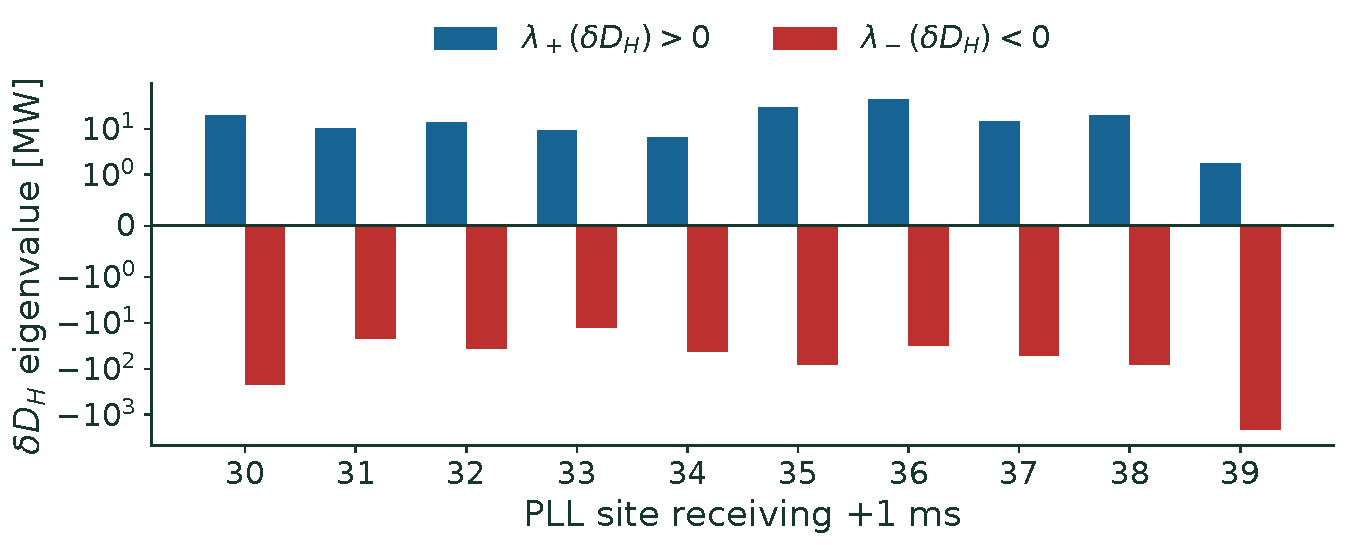
\includegraphics[width=.87\linewidth]{reports/poster/ias2026/collective_interaction_20261003/generated/figures/rank_two.pdf}
\caption{Physical damping redistribution at the preregistered illustrative
frequency 5 Hz, analytical design. One PLL delay is increased from
40 to 41 ms at a time. The symmetric-log scale exposes both signs.
This is a harmonic linear-model check, not a nonlinear stability test.}
\label{fig:rankclosure}
\end{figure}

\subsection{Same replacement, unchanged versus analytical gains}
\status{NUMERICALLY\_VALIDATED}
The missing matched comparator is now executed at the same
$\rho_i=0.876$ and $\tau_i=40$ ms as the analytical candidate.
Its gains remain at the common baseline values.
The canonical method-of-steps solver uses Rodas5P, tolerance $10^{-9}$,
maximum step 0.01 s, and a 60 s event horizon. Both phase-derived
frequency and RoCoF metrics use the canonical 0.5 s window over all
39 bus voltages. The five nominal event magnitudes correspond to
the existing constant-impedance perturbation contract.
Equilibrium residual and gain bounds are checked before execution.

\begin{table}[htbp]\centering\small
\caption{All five matched events. $F$ is peak absolute frequency deviation
in Hz; $R$ is peak absolute RoCoF in Hz/s. A denotes the analytical map;
fixed retains the original gains. All original guards also pass.}
\begin{tabular}{rrrrrl}\toprule
Bus, MW & $F_{\rm fixed}$ & $F_{\rm A}$ & $R_{\rm fixed}$ & $R_{\rm A}$ & Guards\\\midrule
8, -100 & 0.465209 & 0.465412 & 0.138636 & 0.138451 & Pass / Pass\\
16, +100 & 0.446979 & 0.447157 & 0.126583 & 0.126491 & Pass / Pass\\
16, -100 & 0.474417 & 0.474624 & 0.129118 & 0.129044 & Pass / Pass\\
29, +100 & 0.431049 & 0.431226 & 0.128359 & 0.128104 & Pass / Pass\\
29, -100 & 0.444418 & 0.444619 & 0.201209 & 0.200774 & Pass / Pass\\
\\[-2.5mm]\bottomrule
\end{tabular}\label{tab:pairedclosure}
\end{table}

Both designs pass all five events. Analytical retuning increases
frequency excursion by $0.000177$--$0.000207$ Hz and reduces RoCoF
by $0.0000744$--$0.000435$ Hz/s across these cases. Its SG actuator
slack is also slightly smaller. These are small numerical tradeoffs,
not a demonstrated engineering advantage; no refinement study was
performed to turn these small differences into accuracy-certified
performance claims. The purpose of the exact gain map is achieved:
the assigned PLL eigenpair is preserved after the prescribed
replacement step. This matched trial does not show that retuning
was necessary for feasibility, that it maximized replacement, or
that it dominates fixed gains.

\begin{figure}[htbp]\centering
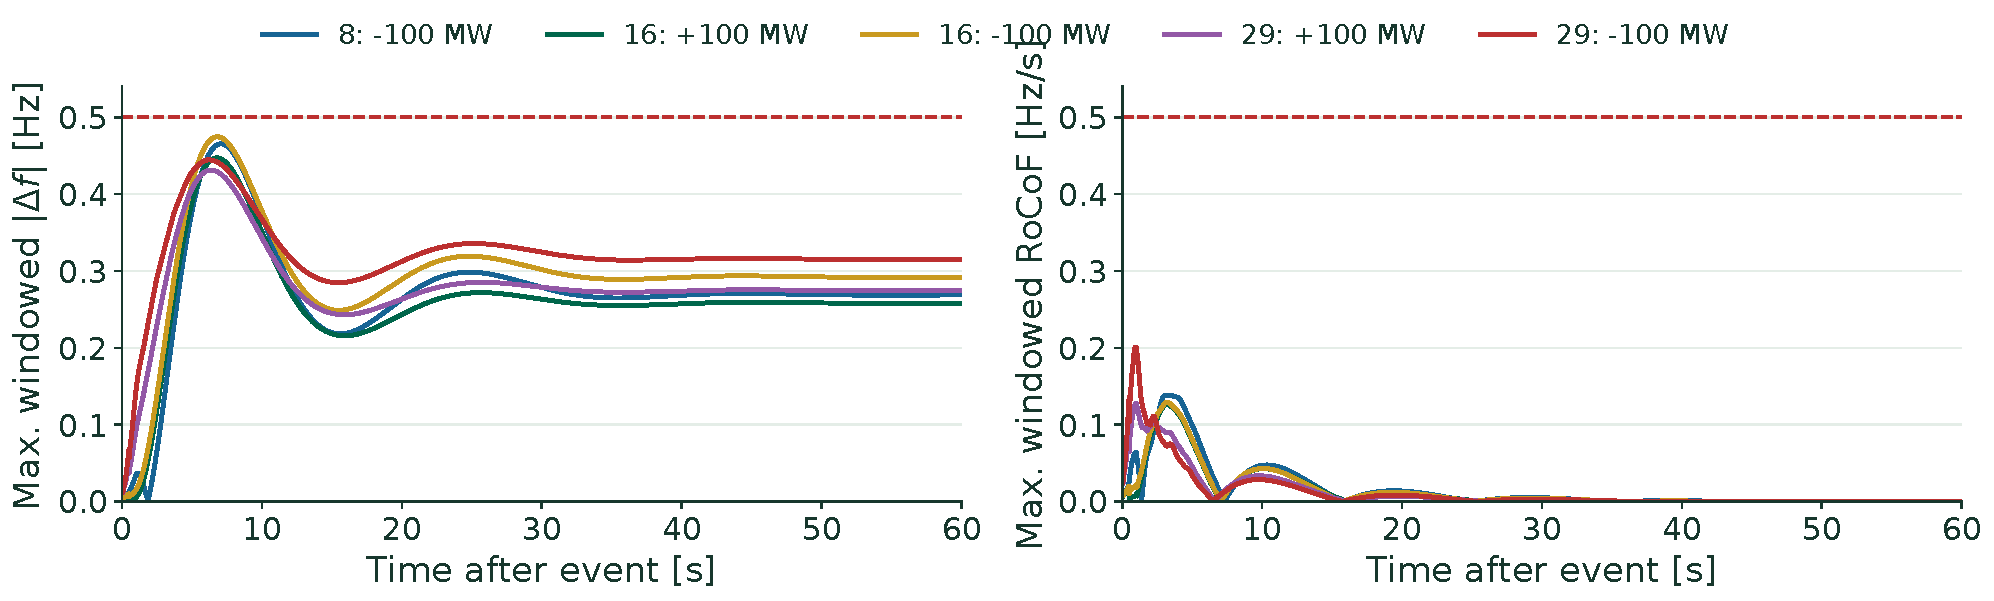
\includegraphics[width=\linewidth]{reports/poster/ias2026/collective_interaction_20261003/generated/figures/events.pdf}
\caption{Preserved analytical-design trajectories for every frozen
event, plotted across the full 60 s horizon. Frequency and RoCoF use
the declared 0.5 s phase window. The new comparator's complete
trajectories and paired metrics are included separately in the archive.}
\label{fig:allfrozen}
\end{figure}

\paragraph{Updated contribution boundary.}
The physical finite-delay theorem, the collective contour Hessian,
and the walk remainder provide explicit equations for network-mediated
effects. The numerical evidence now includes all 60 physical-law
checks and a matched five-event comparator. No informative
verified physical replacement maximum follows. The posterior
comparison therefore supports a theory-and-validation poster;
the stronger application claim remains open.
